\documentclass{article}
\usepackage[utf8]{inputenc}
\usepackage{amssymb}
\usepackage{cite}
\usepackage{subfig}
\usepackage{graphicx}
\usepackage{caption}
\usepackage{float}
\usepackage{amsmath}
\usepackage{listings}
\usepackage{xcolor}
\usepackage{inconsolata}
\usepackage{mdframed}
% \usepackage[portuguese]{babel}
\usepackage[document]{ragged2e}
\usepackage[letterpaper, margin=1.2in]{geometry}


\definecolor{light-gray}{gray}{0.9}

\lstset
{
    % frame=tb, % draw a frame at the top and bottom of the code block
    backgroundcolor = \color{light-gray},
    tabsize=4, % tab space width
    showstringspaces=false, % don't mark spaces in strings
    % numbers=left, % display line numbers on the left
    commentstyle=\color{gray}, % comment color
    keywordstyle=\color{blue}, % keyword color
    stringstyle=\color{red}, % string color
    basicstyle=\footnotesize\ttfamily,
    breaklines=true,
    language=C++,
    literate=   % letters not supported
      {á}{{\'a}}1 {é}{{\'e}}1 {í}{{\'i}}1 {ó}{{\'o}}1 {ú}{{\'u}}1
      {Á}{{\'A}}1 {É}{{\'E}}1 {Í}{{\'I}}1 {Ó}{{\'O}}1 {Ú}{{\'U}}1
      {à}{{\`a}}1 {è}{{\`e}}1 {ì}{{\`i}}1 {ò}{{\`o}}1 {ù}{{\`u}}1
      {À}{{\`A}}1 {È}{{\'E}}1 {Ì}{{\`I}}1 {Ò}{{\`O}}1 {Ù}{{\`U}}1
      {ä}{{\"a}}1 {ë}{{\"e}}1 {ï}{{\"i}}1 {ö}{{\"o}}1 {ü}{{\"u}}1
      {Ä}{{\"A}}1 {Ë}{{\"E}}1 {Ï}{{\"I}}1 {Ö}{{\"O}}1 {Ü}{{\"U}}1
      {â}{{\^a}}1 {ê}{{\^e}}1 {î}{{\^i}}1 {ô}{{\^o}}1 {û}{{\^u}}1
      {Â}{{\^A}}1 {Ê}{{\^E}}1 {Î}{{\^I}}1 {Ô}{{\^O}}1 {Û}{{\^U}}1
      {œ}{{\oe}}1 {Œ}{{\OE}}1 {æ}{{\ae}}1 {Æ}{{\AE}}1 {ß}{{\ss}}1
      {ű}{{\H{u}}}1 {Ű}{{\H{U}}}1 {ő}{{\H{o}}}1 {Ő}{{\H{O}}}1
      {ç}{{\c c}}1 {Ç}{{\c C}}1 {ø}{{\o}}1 {å}{{\r a}}1 {Å}{{\r A}}1
      {€}{{\euro}}1 {£}{{\pounds}}1 {«}{{\guillemotleft}}1
      {»}{{\guillemotright}}1 {ñ}{{\~n}}1 {Ñ}{{\~N}}1 {¿}{{?`}}1
      {ã}{{\~a}}1 {õ}{{\~o}}1 {∆}{{\tiny$\Delta$}}1
      {^}{{\^{}}}1 {±}{{$\pm$}}1
}

\lstnewenvironment{code}[1][C++]
{%
    \mdframed
        [
        backgroundcolor=light-gray, roundcorner=10pt,leftmargin=1, rightmargin=1, innerleftmargin=5, innertopmargin=5,innerbottommargin=5, outerlinewidth=1, linecolor=light-gray
        ]%
    \lstset{
        language=#1
    }
}
{
    \endmdframed
}

\title{Navigation Project}
\author{Tiago Montalvão}

\begin{document}

\maketitle
\justify

\section{Introduction}

This is a report of the first project of Udacity Deep Reinforcement Learning Nanodegree. It describes the model architecture with chosen hyperparameters used in the agent, the experiments, and potential improvements upon the current results.

\section{Implementation}
\subsection{Agent}

The agent was implemented using a Deep Q-Network. To read the paper describing the full details of DQN and from where the following algorithm was taken, see \cite{Mnih2015}.

\begin{figure}[H]
\centering
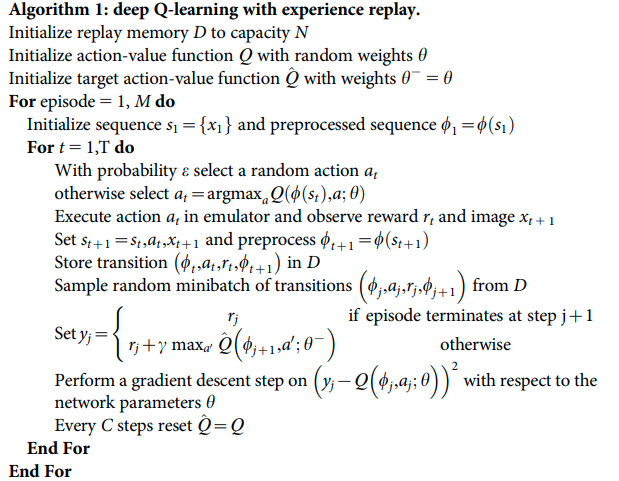
\includegraphics[scale=0.5]{img/DQN.png}
\label{fig:dqn}
\end{figure}

Basically, the DQN consists of a combination of Q-Learning (Sarsamax), which is an off-policy model-free reinforcement learning algorithm, with neural networks, used for approximating the states, since the state space can be huge or sometimes infinite, as it is in this case, since the state gathers some continuous information (e.g. the agent's velocity) 

The DQN was then implemented with:

\begin{itemize}
    \item \textbf{Experience replay buffer} to handle data correlation between consecutive samples.
    \item \textbf{Two neural networks} with identical architecture (local and target networks), as described in the following section, with \textbf{soft update} to the target network.
    \item \textbf{$\varepsilon$-greedy exploration} strategy, with $\varepsilon$ starting at 1.0 and exponentally decreasing up to 0.1.
\end{itemize}

The chosen hyperparametes are described above:

\begin{code}[Python]
BUFFER_SIZE = int(1e5)  # replay buffer size
BATCH_SIZE = 64         # minibatch size
GAMMA = 1.00            # discount factor
TAU = 1e-3              # for soft update of target parameters
LR = 5e-4               # learning rate 
UPDATE_EVERY = 4        # how often to update the network
\end{code}

Here, the discounting factor $\gamma$ was set to 1.0, because there is no need for it to be less than 1 in an episodic task like this.

\subsection{Model architecture}

The model architecture is shown in the figure below:

\begin{figure}[H]
\centering
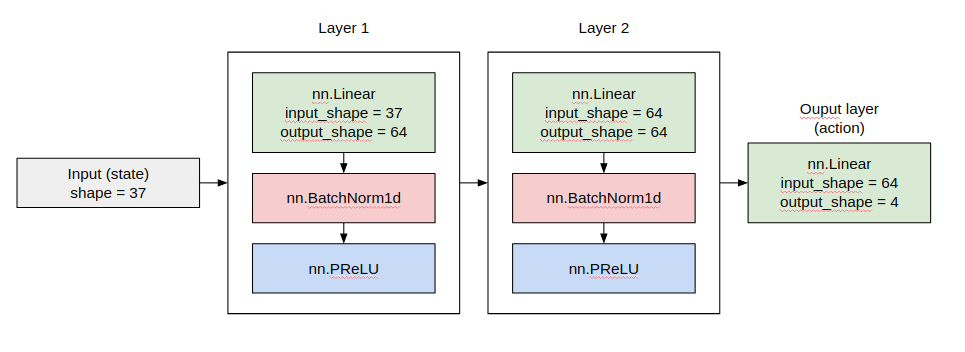
\includegraphics[scale=0.25]{img/model_arch.png}
\label{fig:model_arch}
\end{figure}

There are two hidden layers, each consisting of:

\begin{enumerate}
    \item Linear activation, with 64 neurons
    \item 1d Batch Normalization
    \item Parametric ReLU \cite{he2015delving}
\end{enumerate}

In the project notebook, there is a cell which executes a command that gives the model summary (the same info above with some numbers). The most interesting here is the number of trainable parameters: 7110, which is not large.

\section{Results}

The agent was able to solve the environment in only 848 episodes, and it took it about 32 minutes to train. All the details can be checked in the project notebook.

The following image shows the individual episode score (in blue),the moving average of the last 100 episodes' scores (in orange), and the threshold of 13 for the moving average, so that the environment is considered solved.

\begin{figure}[H]
\centering
\centering
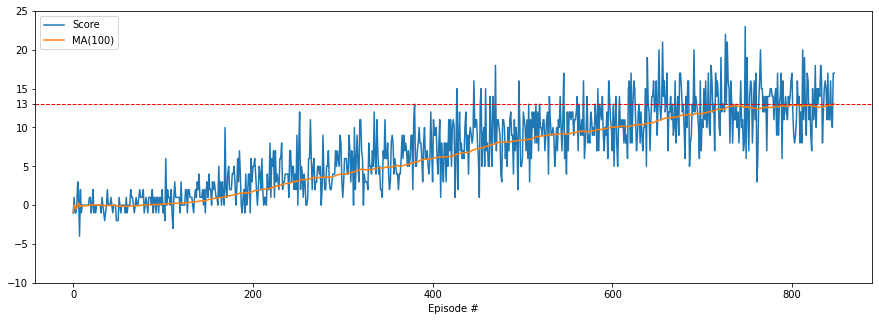
\includegraphics[scale=0.5]{img/score.png}
\label{fig:score}
\end{figure}

It is worth mentioning that, after the training step, $\varepsilon$ was set to 0, so that the agent wouldn't explore and just take the greedy action based on its learned parameters. However, there were times in this scenario in which the agent got stuck, moving forward and backward alternately and effectively staying at the same location. Some of the improvements described in the next section could tackle this problem, such as Prioritized Experience Replay, which could give more weight into sampling this problematic tuple during training.

\section{Ideas for Future Work}

DQN is one of the most classic value-based algorithms for DRL, but a couple of improvements can be implemented. Some of them are:

\begin{itemize}
    \item \textbf{Double DQN} \cite{hasselt2015deep}: tackles the problem of overestimating Q-values.
    \item \textbf{Prioritized Experience Replay} \cite{schaul2015prioritized}: gives more weight in experience sampling from replay buffer for tuples that have larger TD errors.
    \item \textbf{Dueling DQN} \cite{wang2015dueling}: learns a state-value function, along with a function called advantage for each action in a particular state.
\end{itemize}

On top of these improvements and a few more, a new algorithm was developed, called Rainbow \cite{hessel2017rainbow}. In the time this algorithm was developed, it was state-of-the-art.

\bibliography{references}
\bibliographystyle{unsrt}

\end{document}
